\documentclass{article}
\usepackage{authblk}
\usepackage{blindtext}
\usepackage{listings}
\usepackage{color}
\usepackage{amsmath}
\usepackage{amsthm}
\usepackage{graphicx}
\usepackage{amsmath,amssymb,amsthm}
\newcommand{\limp}{\Rightarrow}
\newcommand{\WP}[2]{\mathit{WP}(#1,#2)}
\newcommand{\SP}[2]{\mathit{SP}(#1,#2)}
\newcommand{\havoc}{\mathit{havoc}}
\newcommand{\guard}{\mathit{guard}}
\definecolor{codegreen}{rgb}{0,0.6,0}
\definecolor{codegray}{rgb}{0.5,0.5,0.5}
\definecolor{codepurple}{rgb}{0.58,0,0.82}
\definecolor{backcolour}{rgb}{0.95,0.95,0.92} 
\lstdefinestyle{mystyle}{
    backgroundcolor=\color{backcolour},   
    commentstyle=\color{codegreen},
    keywordstyle=\color{magenta},
    numberstyle=\tiny\color{codegray},
    stringstyle=\color{codepurple},
    basicstyle=\footnotesize,
    breakatwhitespace=false,         
    breaklines=true,                 
    captionpos=b,                    
    keepspaces=true,                 
    numbers=left,                    
    numbersep=5pt,                  
    showspaces=false,                
    showstringspaces=false,
    showtabs=false,                  
    tabsize=2
}
\newtheorem{mydef}{Definition}
\newtheorem{theorem}{Theorem}
\newtheorem{lemma}{Lemma}

\lstset{style=mystyle}
\usepackage[utf8]{inputenc}
\title{Error Localization \& Relevance Analysis \\ }
\author{Matthias Heizmann, Christian Schilling, Numair Mansur}
\affil{University of Freiburg, Germany}
\date{\vspace{-5ex}}
\begin{document}


\begin{mydef}[Execution]\label{mydef:execution_definition}
Let $\pi$ be an error trace of length $n$. An execution of $\pi$ is a sequence of states $s_0, s_1...s_n$ such that $s_i, s_{i+1} \models T$, where $T$ is the transition formula of $\pi[i]$. \\
Let $\epsilon$ represent the set of all possible executions of the error trace.
\end{mydef}

\begin{mydef}[Blocking Execution]\label{mydef:blockingexecution_definition}
An execution of a trace $\pi$ of size $n$ is called a blocking execution if there exists a sequence of states $s_0, s_1...s_j$ where $i<j \leq n$ such that $s_i, s_{i+1} \models T[i]$, where $T[i]$ is the transition formula of $\pi[i]$ and there exits an assume statement in the trace $\pi$ at position $j$ such that $s_{j} \not \limp guard(\pi[j])$.
\end{mydef}

\begin{mydef}[Relevancy of an assignment statement]\label{mydef:relevancy_definition}
Let $\beta$ represent the set of all blocking executions of a trace $\pi$. Let there be an assignment statement of the form $x:=t$ at position $i$. Let $\pi'$ represent the trace that we get after replacing $\pi[i]$ with a havoc statement of the form $havoc(x)$ and let $\beta'$ represent the set of all blocking executions for $\pi'$.\\
We say that the assignment statement $\pi[i]$ is relevant if the trace after the replacement has strictly more blocked executions than the trace before the replacement, i.e if $\beta \subsetneq \beta'$. 
\end{mydef}

\begin{lemma}\label{lemma:duality}
For a program statement $st$ and predicates $P$ and $Q$, where $P$ is condition that is true before the execution of the statement and $Q$ is a post condition, the following two implications are equivilant(also known as the duality of WP and SP):
$$SP(P,st) \Rightarrow Q$$
$$P \Rightarrow WP(Q,st)$$
\end{lemma}

\begin{lemma}[]\label{lemma:rel_bw_assignment_and_havoc}
For a predicate $Q$ and an assignment statement of the form $x:=t$ where $x$ is a variable and $t$ is an expression, we have:
$$WP(Q; havoc(x)) \subseteq WP(Q; x:=t)$$
\end{lemma}

\begin{lemma}[nonempty post]\label{lemma:nonempty_post}
	If $P := \WP{Q}{x := t} \nsubseteq \WP{Q}{\havoc(x)}$ for some $Q$ then $Q \subsetneq \SP{P}{\havoc(x)}$.
\end{lemma}
\begin{proof}
	We will show that $Q \equiv \SP{P}{x := t} \subseteq \SP{P}{\havoc(x)} \not\subseteq Q$ from which it follows that the first inclusion is strict.
	The first inclusion is immediate from Lemma~\ref{lemma:rel_bw_assignment_and_havoc}.
	By assumption $P \not\subseteq \WP{Q}{\havoc(x)}$, which by Lemma~\ref{lemma:duality} is equivalent to the second part.
\end{proof}

\begin{lemma}[restrictiveness]\label{lemma:spfalse}
	If the last statement of a trace $\pi$ of length $n$ is an assume statement and $P \limp \WP{\bot}{\pi}$, then $\SP{P}{\pi[0, j-1]} \not\limp \guard(\pi[j])$ for some $1 \leq j \leq n$.
\end{lemma}
\begin{proof}
	Induction over $n$ (length of $\pi$):
	For $n = 1$ we have $\WP{\bot}{\pi[0]} \equiv \guard(\pi[1]) \limp \bot \equiv \neg \guard(\pi[1])$.
	Now let $n > 1$ and let $Q := \WP{\bot}{\pi[1, n]}$.
	By induction hypothesis $\SP{Q}{\pi[1, j]} \not\limp \guard(\pi[j])$ for some $j$.
	If $\pi[0]$ is an assignment or havoc statement we just apply the hypothesis.
	If $\pi[0]$ is an assume statement then $P \equiv \guard(\pi[1]) \limp Q$, so if $P \not\limp Q$ then $P \not\limp \guard(\pi[1])$.
\end{proof}

\newpage

\begin{theorem}[Relevancy of an assignment statement]\label{mydef:relevancytheorem}
Let $\pi$ be an error trace of length $n$ and $\pi[i]$ be an assignment statement at position $i$ having the form $x:=t$, where $x$ is a variable and $t$ is an expression. Let $P$ and $Q$ be two predicates where $P = \neg WP(False; \pi[i,n]) \cap SP(True; \pi[1, i-1])$ and $Q =  \neg WP(False; \pi[i+1,n])$. The statement $\pi[i]$ is relevant iff:
 $$P \not \limp WP(Q,havoc(x))$$
\end{theorem}

\begin{proof}
Let $\pi'$ be the trace where the assignment statement $\pi[i]$ is replaced by a havoc statement. \\
Note that here we can also write $P$ as $WP(Q; x:=t) \cap SP(True; \pi[1, i-1])$.\\
Let $Q' := SP(P; havoc(x))$ and $P' := WP(Q;havoc(x)) \cap SP(True; \pi[1, i-1])$. \\
Since from lemma~\ref{lemma:rel_bw_assignment_and_havoc} , we know that 
$$WP(Q; havoc(x)) \subseteq WP(Q; x:=t)$$
and also,
$$WP(Q; havoc(x)) \cap SP(True; \pi[1, i-1])  \subseteq WP(Q; x:=t) \cap SP(True; \pi[1, i-1])$$
therefore:
$$P' \subseteq P$$
For simplicity in the proof, lets ignore the term $SP(True; \pi[1, i-1])$ from $P$ and $P'$. We simplify $P$ and $P'$ to be $WP(Q; x:=t)$ and $WP(Q; havoc(x))$ respectively. \\
\\
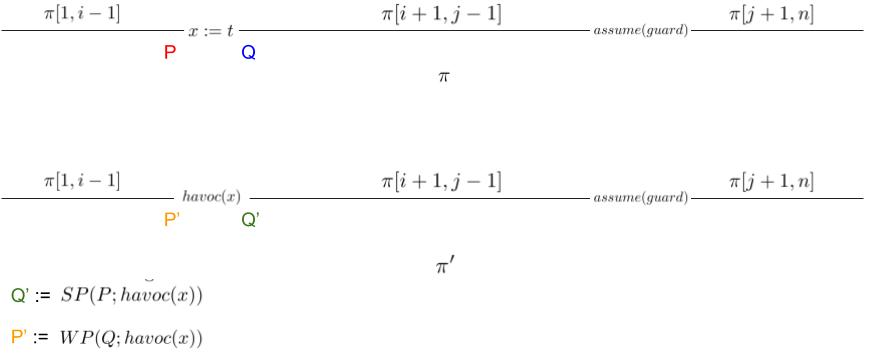
\includegraphics[width=\linewidth]{traces.jpg}\\
"$\Rightarrow$" \\
If the assignment statement $\pi[i]$ is relevant then:
$$P \not \limp WP(Q,havoc(x))$$
Relevancy of $x:=t$ implies that replacing it with $havoc(x)$ gives us strictly more blocking executions then before. Therefore
$$Q \subsetneq Q'$$
\newpage
Lets look at the following diagram to help us see the states a little better and come to the following conculsions:\\
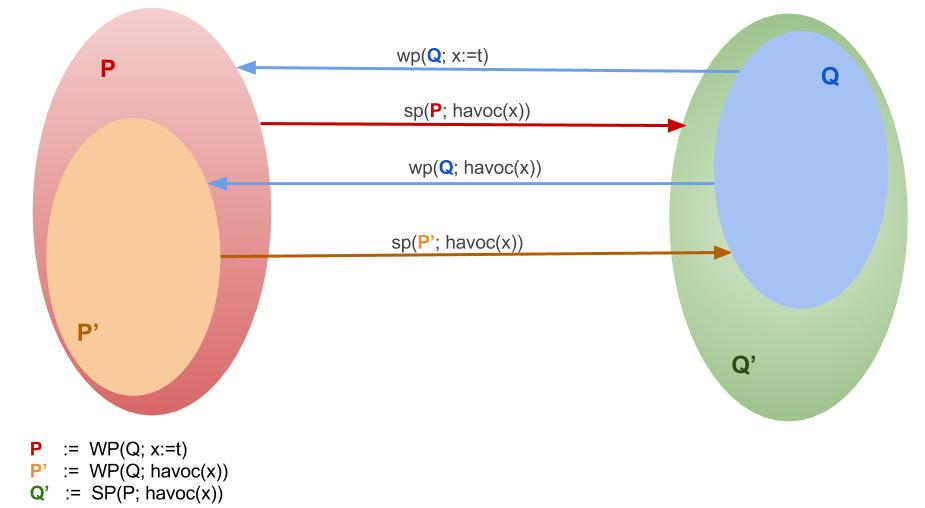
\includegraphics[width=\linewidth]{states.jpg}\\
$$SP(P; havoc(x)) = Q'$$
$$SP(P'; havoc(x)) = Q$$
and we know that $Q \subsetneq Q'$. This means that $\exists S \in P \setminus P'$, such that there is a transition from $S$ to $Q'$ if we execute $havoc(x)$. The existence of the state $S$ means:
$$P \not \limp P'$$
or
$$P \not \limp WP(Q; havoc(x))$$
"$\Leftarrow$"\\
If 
$$P \not \limp WP(Q,havoc(x))$$
then the assignment statement $x:=t$ at position $i$, is relevant.\\
By the definition of $P$:
$$WP(Q; x:=t) \not \limp WP(Q;havoc(x))$$
By lemma~\ref{lemma:nonempty_post}:
$$Q \subsetneq SP(Q; havoc(x))$$
or
$$Q \subsetneq Q'$$
Let $R = Q' \setminus Q$ or $Q' = R \biguplus Q$ (disjoint union of R and Q).\\
Now if we can show that there are states in $R$ such that there is a blocking execution from those states, then that would mean that replacing the assignment with havoc have introduced new blocking execitions. We can show this fact by contradiction. \\
Let us assume that for all $i \leq j \leq n$, statement $\pi[j]$ is not restrictive. i.e
\begin{equation}\label{equation:contradiction}
SP(Q'; \pi[i; j-1]) \limp guard(\pi[j]) \qquad \forall i \leq j \leq n
\end{equation}
We know that
$$SP(X \cup Y; \pi) = SP(X; \pi) \cup SP(Y; \pi)$$
So we can write~\ref{equation:contradiction} as:
$$SP(R; \pi[i; j-1]) \cup SP(Q;\pi[i; j-1]) \limp guard(\pi[j]) \qquad \forall i \leq j \leq n $$
We only have to show the contradiction on $R$
\begin{equation}\label{equation:contradiction_equation}
SP(R; \pi[i; j-1]) \limp guard(\pi[j]) \qquad \forall i \leq j \leq n
\end{equation}
We know that $R \limp \neg Q$, or
\begin{equation}
R \limp WP(false; \pi[i+1,n])
\end{equation}
Considering equation(~\ref{equation:contradiction}) and (~\ref{equation:contradiction_equation}) and lemma(~\ref{lemma:spfalse}), we get a contradiction. That means that we must have atleast one execution which is blocking and hence the statement $x:=t$ is relevant.
\end{proof}
\end{document}